% fig_blocking.tex -- blocking vs nonblocking timing cartoon
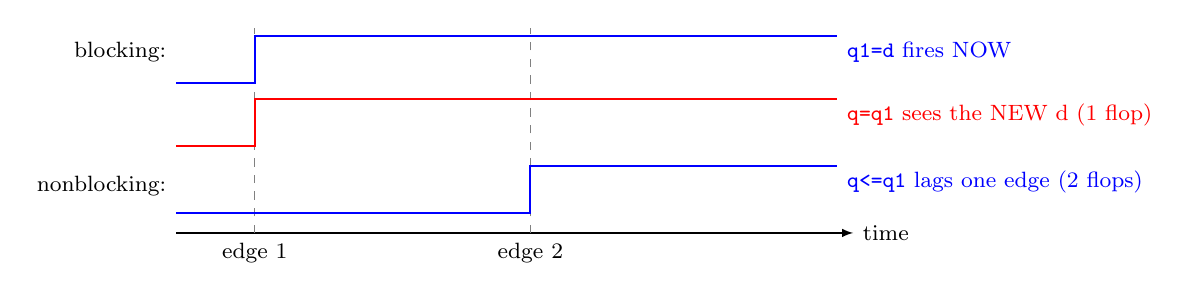
\begin{tikzpicture}[font=\footnotesize, >=latex]
  \draw[->] (0,0) -- (8.6,0) node[right]{time};
  \foreach \x/\l in {1/edge 1, 4.5/edge 2}{
    \draw[dashed, gray] (\x,0) -- (\x,2.6); \node[below] at (\x,0) {\l}; }
  % blocking lane
  \node[left] at (0,2.3) {blocking:};
  \draw[thick, blue] (0,1.9) -- (1,1.9) -- (1,2.5) -- (8.4,2.5);
  \node[right, blue] at (8.4,2.3) {\texttt{q1=d} fires NOW};
  \draw[thick, red] (0,1.1) -- (1,1.1) -- (1,1.7) -- (8.4,1.7);
  \node[right, red] at (8.4,1.5) {\texttt{q=q1} sees the NEW d (1 flop)};
  % nonblocking lane
  \node[left] at (0,0.6) {nonblocking:};
  \draw[thick, blue] (0,0.25) -- (4.5,0.25) -- (4.5,0.85) -- (8.4,0.85);
  \node[right, blue] at (8.4,0.65) {\texttt{q<=q1} lags one edge (2 flops)};
\end{tikzpicture}
